\documentclass[border=2pt]{standalone}
\usepackage{pgfplots}
\usepackage{xcolor}

\pgfplotsset{compat=1.18}

\definecolor{Garnet}{HTML}{73000A}
\definecolor{Gray10}{gray}{0.10}
\definecolor{Gray30}{gray}{0.30}
\definecolor{Gray50}{gray}{0.50}
\definecolor{Gray70}{gray}{0.70}
\definecolor{Gray90}{gray}{0.90}

\pgfplotsset{
  every axis/.style={
    axis line style={draw=black, line width=0.6pt},
    tick style={draw=black, line width=0.6pt},
    tick label style={font=\footnotesize\color{black}},
    label style={font=\small\color{black}},
    grid=both,
    grid style={draw=Gray90, line width=0.3pt},
    legend style={
      draw=none,
      font=\footnotesize\color{black},
      fill=white,
      at={(0.95,0.05)},
      anchor=south east,
    },
  },
  linestyle/.style={
    line width=0.8pt,
    mark=none,
  },
}
\begin{document}


% RF-DETR mAP50
\begin{figure}[h]
\centering
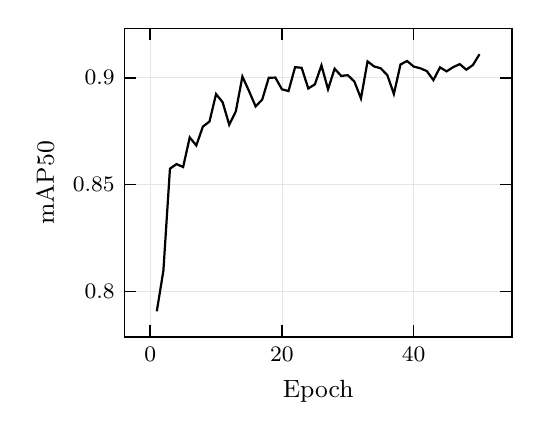
\begin{tikzpicture}
\begin{axis}[
  xlabel={Epoch},
  ylabel={mAP50},
  width=6.5cm,
  height=5.5cm,
]
\addplot[linestyle, color=black] coordinates {
  (1,0.790735)
  (2,0.809700)
  (3,0.857462)
  (4,0.859582)
  (5,0.858226)
  (6,0.872048)
  (7,0.868305)
  (8,0.877125)
  (9,0.879479)
  (10,0.892335)
  (11,0.888519)
  (12,0.877979)
  (13,0.884259)
  (14,0.900513)
  (15,0.893782)
  (16,0.886578)
  (17,0.889688)
  (18,0.899963)
  (19,0.900052)
  (20,0.894563)
  (21,0.893743)
  (22,0.904928)
  (23,0.904607)
  (24,0.894948)
  (25,0.896863)
  (26,0.905755)
  (27,0.894577)
  (28,0.904207)
  (29,0.900808)
  (30,0.901183)
  (31,0.898198)
  (32,0.890310)
  (33,0.907623)
  (34,0.905255)
  (35,0.904393)
  (36,0.901195)
  (37,0.892384)
  (38,0.906174)
  (39,0.907799)
  (40,0.905208)
  (41,0.904396)
  (42,0.903097)
  (43,0.898866)
  (44,0.904818)
  (45,0.902960)
  (46,0.904930)
  (47,0.906341)
  (48,0.903743)
  (49,0.905931)
  (50,0.910975)
};
\end{axis}
\end{tikzpicture}
\end{figure}

% RF-DETR mAP50-95
\begin{figure}[h]
\centering
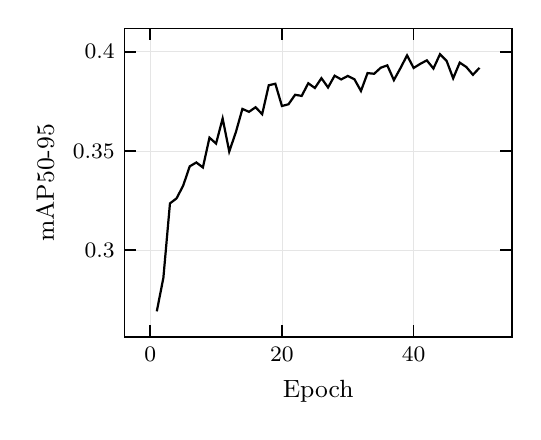
\begin{tikzpicture}
\begin{axis}[
  xlabel={Epoch},
  ylabel={mAP50-95},
  width=6.5cm,
  height=5.5cm,
]
\addplot[linestyle, color=black] coordinates {
  (1,0.269223)
  (2,0.286077)
  (3,0.323611)
  (4,0.326123)
  (5,0.332499)
  (6,0.342263)
  (7,0.344218)
  (8,0.341726)
  (9,0.356714)
  (10,0.353762)
  (11,0.366403)
  (12,0.349726)
  (13,0.359418)
  (14,0.371211)
  (15,0.369729)
  (16,0.372058)
  (17,0.368540)
  (18,0.383122)
  (19,0.383883)
  (20,0.372675)
  (21,0.373543)
  (22,0.378322)
  (23,0.377753)
  (24,0.384129)
  (25,0.381746)
  (26,0.386679)
  (27,0.382021)
  (28,0.387929)
  (29,0.386062)
  (30,0.387810)
  (31,0.386177)
  (32,0.380252)
  (33,0.389253)
  (34,0.388906)
  (35,0.391948)
  (36,0.393138)
  (37,0.385720)
  (38,0.391779)
  (39,0.398188)
  (40,0.391840)
  (41,0.393896)
  (42,0.395673)
  (43,0.391548)
  (44,0.398762)
  (45,0.395431)
  (46,0.386622)
  (47,0.394542)
  (48,0.392308)
  (49,0.388399)
  (50,0.391922)
};
\end{axis}
\end{tikzpicture}
\end{figure}



\end{document}
